%!TEX root = <main.tex>
\section{Introduction}
Deep convolutional neural networks (CNNs) \cite{alexnet, vggnet} have revolutionized the computer vision field with even resulting near-human accuracies for some image recognition challenges.
Many of these successful pre-trained CNNs from computer vision challenges have been successfully repurposed to be used in other real-world image recognition tasks, using a paradigm called \textit{transfer learning} \cite{transfer-learning-factors}.
In transfer learning, instead of training a CNN from scratch, one uses a pre-trained Deep CNN, e.g., ImageNet trained VGG, and fine tune it for the target problem using the target training dataset.
This approach avoids the need for a large training datasets, computational power and time which is otherwise a bottleneck for training a CNN from scratch.
As a result, this paradigm has enabled the wide adoption of deep CNN technology in variety of real world image recognition tasks in several domains including health care \cite{kermany2018identifying, islam2017abnormality}, agriculture \cite{mohanty2016using}, security \cite{arbabzadah2016identifying}, and sociology \cite{wang2017deep}.

% \begin{figure}[ht]
%   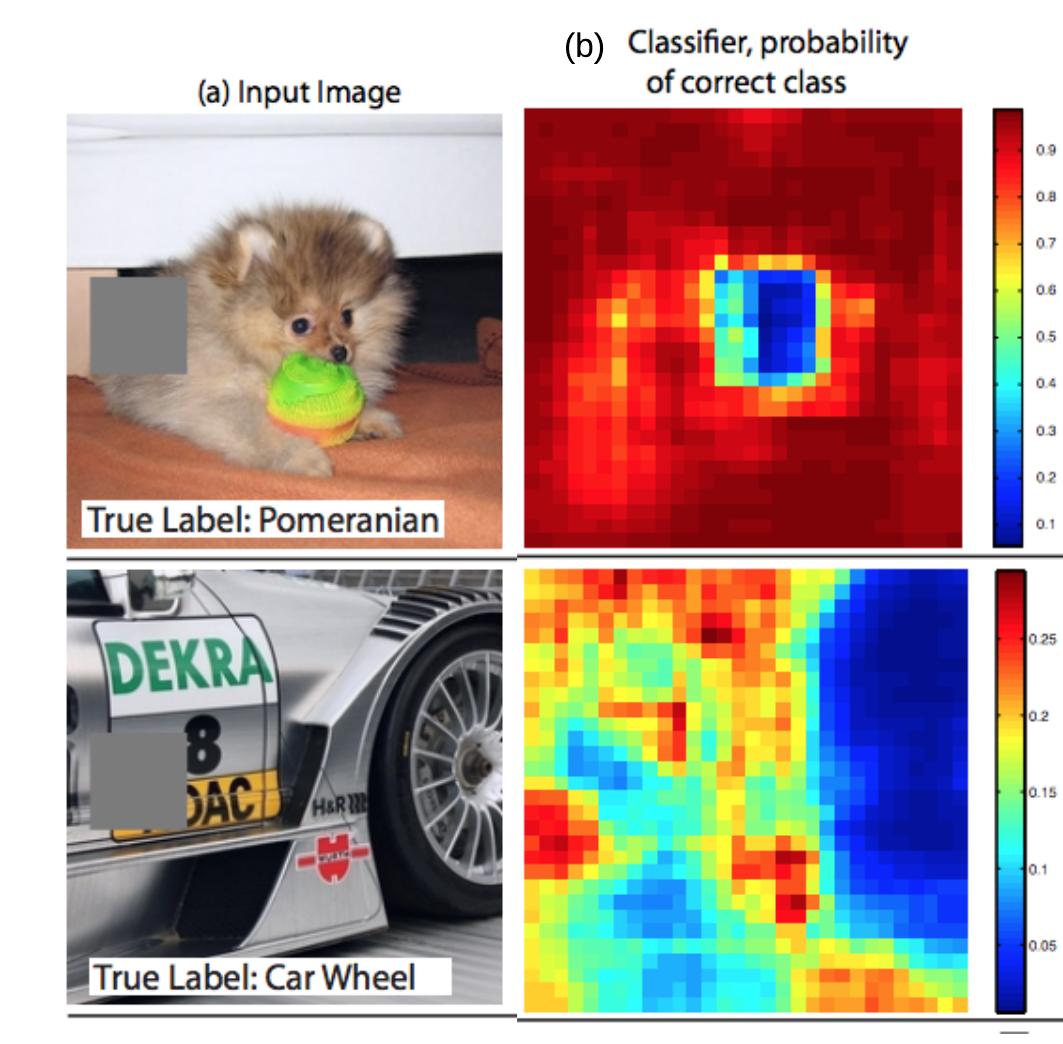
\includegraphics[width=0.9\columnwidth]{./images/occlusion_maps}
%   \caption{Occlusion Experiments (source: \cite{zeiler2014visualizing}).}
%   \label{fig:occlusion_maps}
% \end{figure}

One of the major criticisms for deep CNNs, and deep neural networks in general, is the black-box nature of how they make predictions.
In order to apply deep CNN based techniques in critical applications such as health care, the decisions should be explainable so that the practitioners can use their human judgment to decide whether to rely on those predictions or not \cite{jung2017deep}.
In order to improve the explainability of deep CNN predictions several approaches have been proposed.
One of the most widely used approach in image classification tasks is occlusion experiments \cite{zeiler2014visualizing}.
In occlusion experiments, a square patch, usually of gray or black color, is used to occlude parts of the image and record the variation in the predicted label probability.
By systematically striding this patch horizontally and vertically one or two pixels at a time over the image, a sensitivity heatmap for the predicted label can be generated.
Using this heatmap, the regions in the image which are highly sensitive (or highly contributing) to the predicted class can be identified.
This localization of highly sensitive regions then enables the practitioners to get an idea on the the prediction process of the deep CNN (see Figure. \ref{fig:occlusion_maps}).

However, occlusion experiments are highly compute intensive and time consuming as each patch super imposition is treated as a new image and requires a separate CNN inference.
In this work our goal is to apply database style optimizations to the occlusion based explainability workload to reduce both the computational cost and runtime taken for an experiment.
This will also make occlusion experiments more amenable for interactive diagnosis of CNN predictions.
Our main motivation is based on the observation that when performing CNN inference corresponding to each individual patch position, there are lot of redundant computations which can be avoided.
To avoid redundant computations we introduce the notion of \textit{incremental inference} of deep CNNs which is inspired by the incremental view maintenance approach which is studied to the depth in the context of relational databases.
Due to the overlapping nature of how a convolution kernel would operate, the size of the modified patch will start growing as it progress through more layers in a CNN and reduce the amount of redundant computations.
However at deeper layers the effect over patch coordinates which are radially further away from the center of the patch position will be diminishing.
Our second optimization is based on this observation where we apply a form of approximate inference which applies a \textit{propagation threshold} to limit the growth of the updating patch.
We show that by applying propagation thresholds, a significant amount of computation redundancy can be retained without affecting the perceived quality of the generated sensitivity heatmap.
The third optimization is also a form of approximate inference which we refer as \textit{adaptive drill-down}.
In most occlusion experiment use cases, such as in medical imaging, the object of interest is contained in a relative small region of the image.
In such situations it is unnecessary to inspect the original image at the same high resolution of striding the patch one or two pixels at a time, at all image locations.
In adaptive drill-down approach, first a low resolution heatmap is generated with a larger stride with relatively low computational cost and only the interested regions will be inspected further with a lower stride generating a higher resolution output.
This two stage process also reduces the runtime of occlusion experiments without affecting the accuracy of the occlusion experiment output significantly.

\noindent \textbf{Outline.} The rest of this paper is organized as follows.
